\documentclass[10pt, a4paper]{article}
\usepackage[utf8]{inputenc}
\newcommand\preamble{
    \usepackage[italian]{babel}
    \usepackage{geometry}
    \usepackage{amsmath}
    \usepackage{amssymb}
    \usepackage{graphicx}
    \usepackage{ulem}
    \geometry{margin=2cm}
    \usepackage{listings}
    \usepackage{xparse}
    \usepackage{expl3}
    \usepackage{tikz}
    \usepackage[colorlinks=true, linkcolor=blue]{hyperref}
    \usetikzlibrary{calc}
    \let\olditemize\itemize
    \renewcommand\itemize{\olditemize\setlength\itemsep{0em}}
    \geometry{a4paper, left=1.5cm, right=1.5cm, top=1cm, bottom=2cm}
}
\newcommand{\tikzmark}[1]{\tikz[baseline,remember picture] \coordinate (#1) {};}
\newcommand{\customfbox}[1]{
    \begin{center}
        \noindent\fbox{\parbox{\dimexpr\linewidth-2\fboxsep-2\fboxrule\relax}{\centering #1}}
    \end{center}
    }
\newcommand{\taylor}[3]{
    T_{#2,#3}^{#1}
}
\preamble
\begin{document}
    \begin{center}
        \begin{tabular}{|c|p{6cm}|p{5cm}|}
            \hline
            \textbf{Tipo di Serie} & \textbf{Forma} & \textbf{Comportamento} \\
            \hline
            \textbf{Armonica Generalizzata} & $\displaystyle \sum_{n=1}^{\infty}\frac{1}{n^\alpha}$ & 
                $\begin{cases}
                    \text{Converge} & \text{se }\alpha > 1 \\
                    +\infty & \text{se }\alpha \leq 1
                \end{cases}$ \\
            \hline
            \textbf{Geometrica} & $\displaystyle \sum_{n=0}^{\infty}q^n$ (o $\sum_{n=1}^{\infty}q^n$) & 
                $\begin{cases}
                    \frac{1}{1-q} & \text{se } |q|< 1 \\
                    +\infty & \text{se } q \geq 1 \\
                    \text{Indeterminata} & \text{se } q \leq -1
                \end{cases}$ \\
            \hline
            \textbf{Serie di Funzioni} & $\displaystyle \sum_{n=1}^{\infty}f_n(x)$ & \\
            \hline
            \textbf{Serie di Potenze} & $\displaystyle \sum_{n=0}^{\infty}a_n x^n$ o $\sum_{n=0}^{\infty}a_n x^{(n+1)}$ & \\
            \hline
            \textbf{Serie a segni alterni} & $\displaystyle\sum_{n=1}^{\infty}(-1)^n a_n$ o $\sum_{n=1}^{\infty}(-1)^{n+1} a_n$ & \\
            \hline
            \textbf{Serie a segni positivi} & $\displaystyle\sum_{n=1}^{\infty}a_n$ & \\
            \hline
        \end{tabular}
    \end{center}

\section{Serie di potenze}
    \subsection{Raggio di Convergenza $R$}
        Sia $l = \lim_{n\to\infty} \left|\frac{a_{n+1}}{a_n}\right|$ o $l = \lim_{n\to\infty} \sqrt[n]{|a_n|}$.
        Allora il raggio di convergenza $R$ è dato da:
        \begin{equation*}
            R=\begin{cases}
                +\infty & \text{se } l = 0\\
                \frac{1}{l} & \text{se } l \in (0,+\infty)\\
                0 & \text{se } l = +\infty
            \end{cases}
        \end{equation*}
    \subsection{Insieme di Convergenza Puntuale $I_c$}
        L'insieme di convergenza puntuale si ottiene studiando la convergenza della serie negli estremi dell'intervallo $(-R, R)$.
        \begin{enumerate}
            \item $\sum_{n=0}^{\infty}a_n (\pm R)^n$
            \item L'insieme $I_c$ sarà $(-R,R)$, $[-R,R)$, $(-R,R]$ o $[-R,R]$ a seconda della convergenza agli estremi.
        \end{enumerate}
\section{Convergenza e Divergenza delle Serie Numeriche}
    \subsection{Convergenza Assoluta e Semplice}
        \begin{equation*}
            \sum_{n=1}^{\infty}a_n \text{ converge assolutamente se } \sum_{n=1}^{\infty}\left|a_n\right| \text{ converge.}
        \end{equation*}
        \textbf{Teorema:} Se una serie converge assolutamente $\implies$ converge semplicemente.
    \subsection{Condizione Necessaria di Cauchy per le Serie}
        Data una serie qualsiasi:
        \begin{equation*}
            \lim_{n\rightarrow+\infty}a_n = \begin{cases}
                0 & \Rightarrow \text{la serie \textbf{può} convergere o divergere (caso dubbio)} \\
                \neq 0 \text{ o non esiste} & \Rightarrow \text{la serie \textbf{diverge} sicuramente}
            \end{cases}
        \end{equation*}
        \textbf{Nota:} Questa condizione è \textbf{necessaria ma non sufficiente} alla convergenza della serie.
    
    \newpage
    \subsection{Criteri di Convergenza/Divergenza per Serie a Termini Definitivamente Positivi}
        (\textit{Ovvero $\exists n_0$ tale che $a_n \geq 0$ per ogni $n \geq n_0$})
        \begin{itemize}
            \item \textbf{Criterio del Rapporto} (Utile con fattoriali $n!$ o potenze con $n$ all'esponente):
            Sia $l = \lim_{n\rightarrow +\infty}\frac{a_{n+1}}{a_n}$.
            \begin{enumerate}
                \item Se $l<1 \Rightarrow$ la serie converge.
                \item Se $l>1 \Rightarrow$ la serie diverge.
                \item Se $l=1 \Rightarrow$ il criterio non fornisce informazioni (la serie può convergere o divergere).
            \end{enumerate}

            \item \textbf{Criterio della Radice} (Utile con potenze $n$-esime come $(f(n))^n$):
            Sia $l = \lim_{n\rightarrow+\infty}\sqrt[n]{a_n}$.
            \begin{enumerate}
                \item Se $l<1 \Rightarrow$ la serie converge.
                \item Se $l>1 \Rightarrow$ la serie diverge.
                \item Se $l=1 \Rightarrow$ il criterio non fornisce informazioni.
            \end{enumerate}

            \item \textbf{Criterio del Confronto}: Supponiamo che $0 \leq a_n \leq b_n$ definitivamente.
            \begin{itemize}
                \item Se $\sum b_n$ converge $\Rightarrow$ $\sum a_n$ converge.
                \item Se $\sum a_n$ diverge $\Rightarrow$ $\sum b_n$ diverge.
            \end{itemize}

            \item \textbf{Criterio del Confronto Asintotico}:
            Siano $a_n, b_n > 0$ definitivamente. Sia $L = \lim_{n\rightarrow +\infty}\frac{a_n}{b_n}$.
            \begin{equation*}
                \begin{cases}
                    L \in (0,+\infty) & \Rightarrow \sum a_n \text{ e } \sum b_n \text{ hanno lo stesso comportamento (convergenza/divergenza)} \\
                    L = 0 & \Rightarrow \text{Se } \sum b_n \text{ converge} \Rightarrow \sum a_n \text{ converge (se } \sum b_n \text{ diverge, nulla si può dire)} \\
                    L = +\infty & \Rightarrow \text{Se } \sum b_n \text{ diverge} \Rightarrow \sum a_n \text{ diverge (se } \sum b_n \text{ converge, nulla si può dire)}
                \end{cases}
            \end{equation*}
            \textit{Suggerimento per scegliere $b_n$}: Prendi i termini di grado maggiore in numeratore e denominatore di $a_n$. (Es. $a_n=\frac{n+1}{n^2+3} \Rightarrow b_n=\frac{n}{n^2}=\frac{1}{n}$)
        \end{itemize}

    \subsection{Criteri di Convergenza per Serie a Termini di Segno Alterno}
        \begin{itemize}
            \item \textbf{Criterio di Leibniz} (per serie del tipo $\sum_{n=1}^{\infty}(-1)^n a_n$ o $\sum_{n=1}^{\infty}(-1)^{n+1} a_n$):
            Se la successione $a_n$ soddisfa le seguenti condizioni:
            \begin{enumerate}
                \item $\lim_{n\rightarrow+\infty}a_n=0$
                \item $a_n$ è decrescente definitivamente ($a_{n+1} \leq a_n$ per $n \geq n_0$)
            \end{enumerate}
            allora la serie converge \textbf{semplicemente}.

            \item \textbf{Stima dell'Errore per Serie di Leibniz}:
            Se una serie converge per il criterio di Leibniz a una somma $S$, e $S_N$ è la somma parziale fino all'N-esimo termine, allora l'errore commesso è limitato dal primo termine tralasciato:
            $\left|S - S_N\right| \leq a_{N+1}$.

            \item \textbf{Criterio di Dirichlet (per serie numeriche)}:
            Consideriamo una serie $\sum_{n=1}^{\infty}a_nb_n$. Se valgono le seguenti condizioni:
            \begin{enumerate}
                \item Le somme parziali di $\sum a_n$ sono limitate: $\exists M>0 \mid \left|\sum_{k=1}^{N}a_k\right|\leq M \quad \forall N\geq 1$.
                \item La successione $b_n$ è monotona (crescente o decrescente) definitivamente.
                \item $\lim_{n\rightarrow+\infty}b_n=0$.
            \end{enumerate}
            Allora la serie $\sum_{n=1}^{\infty}a_nb_n$ converge.
            \textit{(Questo criterio è più generale di Leibniz, che è un caso particolare di Dirichlet con $a_n = (-1)^n$ o $(-1)^{n+1}$)}.
        \end{itemize}
    \begin{center}
        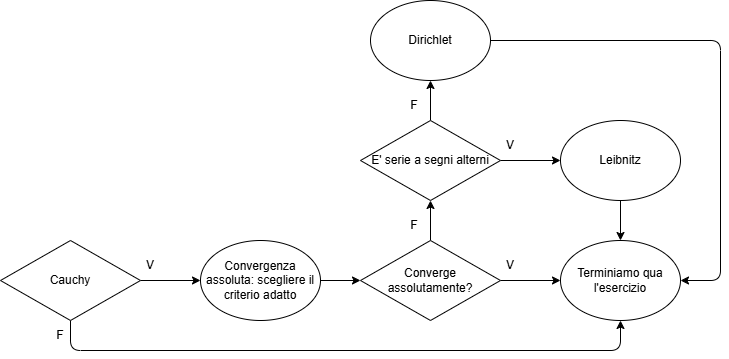
\includegraphics[width=.8\textwidth]{Images/convergenzaflowchart.png}
    \end{center}

    \subsection{Esercizio d'esame}
        \textit{Dire se le seguenti serie convergono semplicemente e/o assolutamente}
        \begin{itemize}
            \item $\displaystyle \sum_{n=1}^{+\infty} \frac{2\sqrt{n}-1}{\binom{2n}{3n}}$ \begin{enumerate}
                \item $\displaystyle \binom{2n}{3n}\sim \frac{1}{\sqrt{2\pi n}}\sqrt{\frac{3}{2}}\left(\frac{27}{4}\right)^n\sim \frac{\sqrt{3}}{\sqrt{4\pi n}}\left(\frac{27}{4}\right)^n\sim\frac{\sqrt{3}}{2\sqrt{\pi n}}\left(\frac{27}{4}\right)^n$
                \item Cauchy: $\displaystyle \lim_{n\to +\infty}\frac{2\sqrt{n}-1}{\binom{2n}{3n}}=\lim_{n\to +\infty}\frac{2\sqrt{n}-1}{\frac{\sqrt{3}}{2\sqrt{\pi n}}\left(\frac{27}{4}\right)^n}=\lim_{n\to +\infty}\frac{4n\sqrt{\pi}-2\sqrt{\pi n}}{\sqrt{3}\left(\frac{27}{4}\right)^n}=0$ verificato
                \item Equivalente asintotico: $\displaystyle \frac{4n\sqrt{\pi}-2\sqrt{\pi n}}{\sqrt{3}\left(\frac{27}{4}\right)^n}\sim \frac{n}{\left(\frac{27}{4}\right)^n}$
                \item Criterio della radice: $\displaystyle \lim_{n\to +\infty}\sqrt[n]{\frac{n}{\left(\frac{27}{4}\right)^n}}=\lim_{n\to +\infty}\left(\frac{n^{\frac{1}{n}}}{\frac{27}{4}}\right)=\frac{1}{\frac{27}{4}}=\frac{4}{27}<1\Rightarrow$ converge assolutamente
            \end{enumerate}
            \item $\displaystyle \sum_{n=2}^{+\infty}(-1)^{n+1}\frac{3n}{n^2-2n+1}$ \begin{enumerate}
                \item Cauchy: $\displaystyle \lim_{n\to +\infty}\frac{3n}{n^2-2n+1}=\frac{+\infty}{+\infty_2}=0$ verificato
                \item Equivalente asintotico: $\displaystyle \frac{3n}{n^2-2n+1}\sim \frac{n}{n^2}\sim\frac{1}{n}\Rightarrow$ non converge assolutamente (serie armonica generalizzata $\alpha\leq 1$)
                \item Leibnitz: \begin{enumerate}
                    \item Cauchy verificato prima
                    \item Decrescente? \begin{equation*}
                        \begin{split}
                            \frac{3n}{(n-1)^2} &\geq \frac{3(n+1)}{((n+1)-1)^2}\\
                            \frac{n}{(n-1)^2} &\geq \frac{(n+1)}{((n+1)-1)^2}\\
                            n &\geq \frac{(n+1)(n-1)^2}{((n+1)-1)^2}\\
                            n((n+1)-1)^2 &\geq (n+1)(n-1)^2\\
                            n^2+n-1&\geq 0\\
                            n_{1,2}&=\frac{-1\pm\sqrt{5}}{2}\rightarrow \text{decrescente da qua in poi}
                        \end{split}
                    \end{equation*}
                    \item Soddisfa entrambi i requisiti quindi converge semplicemente
                \end{enumerate}
            \end{enumerate}
            \item \textit{Determinare l'insieme di convergenza puntuale $I$ della serie di potenze}   $\displaystyle \sum_{n=1}^{+\infty}\frac{n}{5^n}x^n$ \begin{enumerate}
                \item Cauchy: $\displaystyle \frac{n}{5^n}=0$
                \item Criterio della radice: $\displaystyle \lim_{n\to +\infty}\sqrt[n]{\left|\frac{n}{5^n}\right|}=\lim_{n\to +\infty}\frac{n^\frac{1}{n}}{5}=\frac{1}{5}$
                \item $\displaystyle R=\frac{1}{\frac{1}{5}}=5$
                \item $\displaystyle\sum \frac{n}{5^n}(-5)^n=\sum -n \qquad \lim_{n\to +\infty}|-n|=+\infty$
                \item $\displaystyle\sum \frac{n}{5^n}5^n=\sum n \qquad \lim_{n\to +\infty}n=+\infty$
                \item $I=(-5,5)$
            \end{enumerate}
        \end{itemize}
\section{Polinomio di McLaurin}
    Consideriamo:
    \begin{equation*}
        c_k = \frac{f^{(k)}(0)}{k!}
    \end{equation*}
    \begin{equation*}
        f^{(k)}(0) = c_k\cdot k!
    \end{equation*}
    \begin{equation*}
        P_k(x)=f(0)+\sum_{n=1}^{k}c_k x^k
    \end{equation*}
    \begin{center}
        \begin{tabular}{|p{4cm}|p{10.5cm}|}
            \hline
            \textbf{Funzione $f(x)$} & \textbf{Serie di Maclaurin} \\
            \hline
            $e^x$ & $\displaystyle \sum_{n=0}^{\infty} \frac{x^n}{n!} = 1 + x + \frac{x^2}{2!} + \frac{x^3}{3!} + \dots$ \\
            \hline
            $\sin(x)$ & $\displaystyle \sum_{n=0}^{\infty} \frac{(-1)^n}{(2n+1)!}x^{2n+1} = x - \frac{x^3}{3!} + \frac{x^5}{5!} - \frac{x^7}{7!} + \dots$ \\
            \hline
            $\cos(x)$ & $\displaystyle \sum_{n=0}^{\infty} \frac{(-1)^n}{(2n)!}x^{2n} = 1 - \frac{x^2}{2!} + \frac{x^4}{4!} - \frac{x^6}{6!} + \dots$ \\
            \hline
            $\frac{1}{1-x}$ (Serie Geometrica) & $\displaystyle \sum_{n=0}^{\infty} x^n = 1 + x + x^2 + x^3 + \dots$ \\
            \hline
            $\ln(1+x)$ & $\displaystyle \sum_{n=1}^{\infty} \frac{(-1)^{n+1}}{n}x^n = x - \frac{x^2}{2} + \frac{x^3}{3} - \frac{x^4}{4} + \dots$ \\
            \hline
            $\arctan(x)$ & $\displaystyle \sum_{n=0}^{\infty} \frac{(-1)^n}{2n+1}x^{2n+1} = x - \frac{x^3}{3} + \frac{x^5}{5} - \frac{x^7}{7} + \dots$ \\
            \hline
            $(1+x)^\alpha$ (Serie Binomiale) & $\displaystyle \sum_{n=0}^{\infty} \binom{\alpha}{n}x^n = 1 + \alpha x + \frac{\alpha(\alpha-1)}{2!}x^2 + \dots$ \\
            & \quad dove $\binom{\alpha}{n} = \frac{\alpha(\alpha-1)\dots(\alpha-n+1)}{n!}$ \\
            \hline
            $(1-x)^{-k}$ & $\displaystyle \sum_{n=0}^{\infty} \binom{n+k-1}{n}x^n = 1 + kx + \frac{k(k+1)}{2!}x^2 + \dots$ \\
            & (Questo è un caso speciale della serie binomiale con $\alpha = -k$) \\
            \hline
        \end{tabular}
    \end{center}
    \subsection{Trovare $f^{(n)}(0)$ con $n$ molto grande}
        \begin{enumerate}
            \item Scomponi $f(0)$ in funzioni le cui serie di McLaurin sono note e riscrivile come sommatorie (praticamente copia e incolla dalla tabella adattando l'argomento)
            \item Prendi il coefficiente di ordine $n$ di ogni sommatoria e poi sommali per ottenere il coefficiente totale
            \item Sapendo la formula del coefficiente $c_k$ dobbiamo isolare $f^{(k)}(0)$ moltiplicando entrambi i lati per $k!$
        \end{enumerate}
        \textit{Esempio: calcolare $f^{(15)}(0)$ di $f(x)=e^{2x}-\frac{x^2}{1+x}$}
        \begin{enumerate}
            \item $e^{2x}\rightarrow\sum_{n=0}^{\infty}\left(\frac{(2x)^n}{n!}\right)\xrightarrow{n=15}\frac{(2x)^{15}}{15!}$
            \item $\frac{x^2}{1+x}\rightarrow\sum_{n=0}^{\infty}\left((-x)^n\cdot x^2\right)=\sum_{n=0}^{\infty}\left((-1)^n\cdot x^n\cdot x^2\right)=\sum_{n=0}^{\infty}\left((-1)^n\cdot x^{n+2}\right)\xrightarrow{n=13} -x^{15}$
            \item $a_{15}=\frac{2^{15}}{15!}x^{15}+x^{15}=x^{15}\left(\frac{2^{15}}{15!}+1\right)\xrightarrow{\text{togliamo le x}} \frac{2^{15}}{15!}+1$
            \item $f^{(15)}(0)=15!\cdot a_{15}=2^{15}\cdot 15!$
        \end{enumerate}
    \subsection{Resto di Lagrange}
        Per trovare il resto di Lagrange di ordine $k$ con centro $x_0$ (solitamente è 0) di una funzione $g(x)$:
        $$
            R_k(x) = \frac{g''(x)}{(k+1)!}x^{(k+1)}
        $$
        Per fare una stima in un intervallo $x\in I$:
        \begin{enumerate}
            \item $|g''(x)|\leq M$
            \item $M$ è la sommatoria di tutti gli elementi di $g''(x)$ a modulo, è possibile usare la disuguaglianza triangolare: $|x-y|\leq |x|+|y|$
            \item Troviamo gli equivalenti asintotici di $M$
            \item Sostituiamo $x$ con il valore di $I$ più grande che possiamo usare
            \item La stima è $\displaystyle |R_k(x)|\leq \frac{M}{(k+1)!}x^{(k+1)}$
        \end{enumerate}
        \subsection{Esercizio da esame}
        \begin{itemize}
            \item \textit{Data la funzione $f(x)=x(e^x-1)+\ln(1+x^2)+\sin(2x)$, calcolarne il polinomio di McLaurin di ordine 4} \begin{enumerate}
                \item Dividiamo $f(x)$ in polinomi che contengono le funzioni elementari quindi avremo: \begin{itemize}
                    \item $x(e^x-1)=x\left(1+x+\frac{1}{2}x^2+\frac{1}{3!}x^3-1\right)=x^2+\frac{x^3}{2}+\frac{x^4}{3!}+o\left(x^4\right)$
                    \item $\ln(1+x^2)=\left(x^2-\frac{(x^2)^2}{2}\right)=x^2-\frac{x^4}{2}+o\left(x^4\right)$
                    \item $\sin(2x)=2\left(x-\frac{x^3}{3!}\right)=2x-\frac{(2x)^3}{3!}+o\left(x^4\right)$
                \end{itemize}
                \item Costruiamo una tabella di questo tipo: 
                \begin{center}
                    \begin{tabular}{| c | c | c | c | c |}
                        \hline
                        \textbf{Ordine} & $x(e^x-1)$ & $\ln(1+x^2)$ & $\sin(2x)$ & \textbf{Somma}\\
                        \hline
                        1 & / & / & $2x$ & $2x$ \\
                        \hline
                        2 & $x^2$ & $x^2$ & / & $2x^2$\\
                        \hline
                        3 & $\frac{x^3}{2}$ & / & $-\frac{(2x)^3}{3!}$ & $-\frac{5x^3}{6}$\\
                        \hline
                        4 & $\frac{x^4}{3!}$ & $-\frac{x^4}{2}$ & / & $-\frac{x^4}{3}$\\
                        \hline
                    \end{tabular}
                \end{center}
                Dove andiamo a prendere gli elementi di ciascun polinomio dell'ordine indicato nella prima colonna ed eseguiamo la somma della riga nell'ultima colonna.
                \item Poi costruiamo il polinomio $P_4(x)$ sommando l'ultima colonna: $P_4(x)=2x+2x^2-\frac{5x^3}{6}-\frac{x^4}{3}$
            \end{enumerate}
            \item \textit{Scrivere il resto di Lagrange $R_1(x)$ di ordine 1 (con centro in 0) della funzione $g(x)=\cos(x^2)+\sin(3x)$ e determinarne una stima per $x\in(0,\frac{1}{4}]$} \begin{enumerate}
                \item $g''(x)=\frac{d}{dx}(g'(x))=-4x^2\cos(x^2)-2\sin(x^2)-9\sin(3x)$
                \item $R_1(x)=\frac{g''(x)}{2!}x^2$
                \item \begin{equation*}
                    \begin{split}
                        &\left|g''(x)\right|\leq M\\
                        &\left|-4x^2\cos(x^2)-2\sin(x^2)-9\sin(3x)\right|\leq \left|4x^2\cos(x^2)\right|+\left|2\sin(x^2)\right|+\left|9\sin(3x)\right|\\
                    \end{split}
                \end{equation*}
                \item Troviamo gli equivalenti asintotici per i singoli elementi di $M$ \begin{equation*}
                    \begin{split}
                        &\sin(x^2)\sim x^2\\
                        &\sin(3x) \sim 3x\\
                        &\cos(x^2) \sim 1 \rightarrow \text{Usiamo 1 perchè vogliamo fare una stima grossolana}
                    \end{split}
                \end{equation*}
                \item Riscriviamo $M$: \begin{equation*}
                    \left|4x^2\cos(x^2)\right|+\left|2\sin(x^2)\right|+\left|9\sin(3x)\right|=4x^2+2x^2+27x=6x^2+27x
                \end{equation*}
                \item Sostituiamo $x=\frac{1}{4}$ perchè è la $x$ più grande che possiamo usare: \begin{equation*}
                    \frac{3}{8}+\frac{27}{4}=\frac{57}{8}
                \end{equation*}
                \item Quindi: \begin{equation*}
                    \left|R_1(x)\right|\leq \frac{M}{2!}x^2\rightarrow\frac{57}{8}\frac{1}{2}x^2=\frac{57}{16}x^2\simeq 3.56x^2
                \end{equation*}
            \end{enumerate}
        \end{itemize}
        \subsection{Esercizio da esame}
        \textit{Calcolare lo sviluppo di Taylor di ordine 8 attorno ad $x_0=0$ della funzione $f(x)=\ln(\cos(x^2))$. Quanto vale $f^{(8)}(0)?$}
        \begin{enumerate}
            \item $\displaystyle \cos(x)=1-\frac{x^2}{2!}+\frac{x^4}{4!}-\frac{x^6}{6!}+\frac{x^8}{8!}+O(x^{10})$
            \item $\displaystyle \cos(x^2) = 1-\frac{x^4}{2!}+\frac{x^8}{4!}+O(x^{12})$
            \item $\displaystyle \ln(1+x)=x-\frac{x^2}{2}+\frac{x^3}{3}-\frac{x^4}{4}+\frac{x^5}{5}-\frac{x^6}{6}+\frac{x^7}{7}-\frac{x^8}{8}+O(x^9)$
            \item $\displaystyle \ln(1+cos(x^2)-1)=-\frac{x^4}{2!}+\frac{x^8}{4!}-\frac{1}{2}\left(\frac{x^4}{2!}+\frac{x^8}{4!}\right)^2+\ldots=-\frac{x^4}{2}+\frac{x^8}{24}-\frac{x^8}{8}+O(x^12)\rightarrow P_8(x)$
            \item $\displaystyle c_8=x^8\left(\frac{1}{24}-\frac{1}{8}\right)=-\frac{1}{12}x^8$
            \item $\displaystyle f^{(8)}(0)=-\frac{1}{12}\cdot 8!=-3360$
        \end{enumerate}
\section{Formula di Taylor}
    \customfbox{$f^{(n)}$ indica l'ordine di derivazione $n$-esimo}
    Data una funzione $f:I\rightarrow\mathbb{R}$ definita su un intervallo $I$ e derivabile infinite volte ($C^{\infty}$)
    \subsection{Polinomio di Taylor di $f$ centrato in $x_0$ di ordine $n$}
        \begin{equation*}
            \taylor{f}{x_0}{n}(x) = f(x_0)+f'(x_0)(x-x_0)+f''(x_0)\frac{(x-x_0)^2}{2!}+\ldots+f^{(n)}(x_0)\frac{(x-x_0)^n}{n!}
        \end{equation*}
    \subsection{Formula di Taylor con resto di Lagrange}
        \begin{equation*}
            \begin{split}
                &f(x) = \taylor{f}{x_0}{n}(x) + R_nf(x)\\
                &R_nf(x) = \frac{f^{(n+1)}(c_n)(x-x_0)^{n+1}}{(n+1)!} \text{ con } c_n\in\{x_0,x\}
            \end{split}
        \end{equation*}
        Se $x=b$ e $x_0$ è vicino a $b$, $\taylor{f}{x_0}{n}(b)$ approssima $f(b)$ e $\left|f(b)-\taylor{f}{x_0}{n}(b)\right| = \left|R_nf(b)\right|$
        \subsubsection{Determinare una stima del resto di Lagrange}
            Se dobbiamo calcolarlo con $x\in(0,a]$ al posto della $x$ negli argomenti delle sotto-funzioni ci mettiamo $a$ e calcoliamo $M$ in base a quello.
            \begin{equation*}
                \left|f^{(k+1)}(c)\right|\leq M
            \end{equation*}
            Dove $M$ è il maggiorante quindi prendiamo tutte le "sotto-funzioni" di $f^{(k+1)}(x)$ e combiniamo tutti i maggioranti tra di loro oppure calcoliamo $f^{(k+1)}(a)$. Per calcolare la stima quindi:
            \begin{equation*}
                \left|R_k(x)\right|\leq \frac{M}{(k+1)!}x^{k+1}
            \end{equation*}
            \textit{Esempio:}
            \begin{equation*}
                \left|f''(x)\right|=\left|e^{-2x}\cdot 13\sin(3x+\phi)\right|
            \end{equation*}
            I valori maggioranti di questi sono $1$ e $13$ (perchè la funzione seno oscilla tra $-1$ e $1$ ma stiamo usando il modulo). Quindi:
            \begin{equation*}
                M = 1\cdot 13 = 13
            \end{equation*}
            Oppure calcoliamo $\left|f''(a)\right|$ per trovare $M$.
            \begin{equation*}
                \left|R_1(x)\right|\leq \frac{M}{2!}x^2
            \end{equation*}
    \subsection{Formula di Taylor con resti di Peano}
        \begin{equation*}
                f(x)= \taylor{f}{x_0}{n}(x) + (x-x_0)^n + \varepsilon(x-x_0) \text{ con } \lim_{x\rightarrow x_0} \varepsilon(x-x_0) = 0
        \end{equation*}
    \subsection{Stimare l'errore commesso}
        $$
        |R_k(x_0)|=|T_k(x_0)-f(x_0)|
        $$
    \subsection{Unicità del Polinomio di Taylor}
    \begin{equation*}
        f(x)=(a_0+a_1(x-x_0)+\ldots+a_n(x-x_0)^n)+\varepsilon(x-x_0)(x-x_0)^n
    \end{equation*}
    Dove $a_0,a_1,\ldots,a_n\in\mathbb{R}$ e $\lim_{x\rightarrow x_0}\varepsilon(x-x_0)=0$ allora:
    \begin{equation*}
        a_k = \frac{f^{(k)}(x_0)}{k!}
    \end{equation*}
\newpage
\section{Fourier}
    \subsection{Coefficienti}
        Data una funzione $f$ periodica di periodo $T$, i coefficienti di Fourier sono dati da:
        \begin{equation*}
            \hat{f_k}=\frac{1}{T}\int_{-\frac{T}{2}}^{\frac{T}{2}}f(x)e^{-i\frac{2\pi}{T}kx} \qquad k\in\mathbb{Z}
        \end{equation*}
        E usando l'identità di Eulero:
        \begin{equation*}
            \hat{f_k}=\left(\frac{1}{T}\int_{-\frac{T}{2}}^{\frac{T}{2}}f(x)\cos\left(\frac{2\pi}{T}kx\right)dx\right)-i\left(\frac{1}{T}\int_{-\frac{T}{2}}^{\frac{T}{2}}f(x)\sin\left(\frac{2\pi}{T}kx\right)dx\right)
        \end{equation*}
        \subsubsection{Coefficienti reali}
        \begin{itemize}
            \item $a_k=\hat{f_k}+\hat{f}_{-k}=\frac{2}{T}\int_{-\frac{T}{2}}^{\frac{T}{2}}f(x)\cos\left(\frac{2\pi}{T}kx\right)dx$
            \item $b_k=i(\hat{f_k}+\hat{f}_{-k})=\frac{2}{T}\int_{-\frac{T}{2}}^{\frac{T}{2}}f(x)\sin\left(\frac{2\pi}{T}kx\right)dx$
        \end{itemize}
        \textbf{Proprietà:} \begin{itemize}
            \item Se $f(x)$ è pari $\Rightarrow b_k$ nulli
            \item Se $f(x)$ è dispari $\Rightarrow a_k$ nulli tranne $a_0=0$
        \end{itemize}
    \subsection{Serie di Fourier}
        \begin{equation*}
            f(x)\sim \frac{a_0}{2}+\sum_{k=1}^{+\infty}\left[a_k\cos\left(\frac{2\pi k}{T}x\right)+b_k\sin\left(\frac{2\pi k}{T}x\right)\right]
        \end{equation*}
    \subsection{Criterio di Dirichlet}
        Permette di dire a cosa converge e/o a dire il \textbf{valore della serie} di Fourier.
        $$
        \tilde{f}(x)=\begin{cases}
            f(x) & \text{se continua}\\
            \frac{f(x^+)+f(x^-)}{2} & \text{se discontinua in } x
        \end{cases}
        $$
        \subsubsection{Utilizzo}
        \begin{enumerate}
            \item Se la funzione è definita a tratti cerchiamo i punti di giunzione e controlliamo se sono continui o no (usando la tecnica del limite sinistro e destro), se la funzione è periodica anche gli estremi devono essere considerati come punti di giunzione            \item Riscrivi $\tilde{f}(x)$ impostando la condizione (se periodica di periodo $T$) come $x=x_0+Tk$ o $x\neq x_0+Tk$ dove $x_0$ è il punto di discontinuità
        \end{enumerate}
    \customfbox{Una serie di Fourier converge \textbf{uniformemente} se $f$ è continua su tutto $\mathbb{R}$ (o su $T$). Per vedere se una serie converge uninformemente basta usare una di queste strategie: \begin{itemize}
        \item Funzione continua e derivabile a tratti $\Rightarrow$ converge
        \item Usare il criterio di Weierstrass
        \item E' funzione Lipschitziana ($|f(x)-f(y)|\leq k|x-y|$)
    \end{itemize}}
    \subsection{Esercizio d'esame}
    \textit{Sia $f$ la funzione ottenuta estendendo per periodicità a tutto $\mathbb{R}$ la funzione} \begin{equation*}
        g(x)=\begin{cases}
            2\pi + x & x\in[-\pi,0)\\
            2\pi - x & x\in[0,\pi)\\
        \end{cases}
    \end{equation*}
    \begin{itemize}
        \item \textit{Disegna il grafico di $f$}
        \item \textit{Calcolare il coefficiente di Fourier $\hat{f_0}$} \begin{enumerate}
            \item Sappiamo che $\hat{f_0}=\frac{1}{2\pi}\int_{-\pi}^{\pi}f(x)dx=\frac{1}{2\pi}\left[\int_{-\pi}^{0}(2\pi+x)dx+\int_{0}^{\pi}(2\pi-x)dx\right]=\frac{3\pi}{2}$
        \end{enumerate}
        \item \textit{Calcolare il coefficiente di Fourier $\hat{f_k}$ per $k\neq 0$} \begin{enumerate}
            \item Se $f(x)$ è pari, i coefficienti $b_k$ sono nulli e i coefficienti $a_k=\frac{2}{2\pi}\int_{-\pi}^{\pi}f(x)\cos(\frac{2\pi}{2\pi}kx)dx=\frac{2}{\pi}\int_{0}^{\pi}f(x)\cos(kx)dx$
            \item Poichè $\hat{f_k}=\frac{a_k-ib_k}{2}$ nel nostro caso sarà $\hat{f_k}=\frac{a_k}{2}$
            \item Calcoliamo $a_k$ \begin{equation*}
                a_k = \frac{2}{\pi}\int_{0}^{\pi}(2\pi-x)\cos(kx)dx=\frac{2}{\pi k^2}[1-(-1)^k]
            \end{equation*}
            \item Quindi dobbiamo calcolare per $k$ pari e $\neq 0$ e dispari: \begin{equation*}
                \hat{f_k}=\begin{cases}
                    \frac{2}{\pi k^2} & \text{se } k \text{ dispari}\\
                    0 & \text{se } k \text{ pari e } \neq 0
                \end{cases}
            \end{equation*}
        \end{enumerate}
        \item \textit{Calcolare il valore della serie di Fourier di $f$ sull'intervallo $[-\pi,\pi)$} \begin{enumerate}
            \item Sappiamo che $T=2\pi$
            \item Calcoliamo $a_0$: \begin{equation*}
                \begin{split}
                    a_0 &= \frac{2}{T}\int_{-\frac{T}{2}}^{\frac{T}{2}}f(x)dx=\frac{2}{\pi}\int_{0}^{\pi}(2\pi-x)dx=\frac{2}{\pi}\left(\int_{0}^{\pi}2\pi dx-\int_{0}^{\pi}x dx\right)\\
                    &=\frac{2}{\pi}\left(2\pi\left[x\right]_{0}^{\pi}-\left[\frac{x^2}{2}\right]_{0}^{\pi}\right)=\frac{2}{\pi}\left(2\pi^2-\frac{\pi^2}{2}\right)=\frac{2}{\pi}\frac{3\pi^2}{2}=3\pi
                \end{split}
            \end{equation*}
            \item Sostituiamo $a_0, a_k \text{ e } b_k$ con quelli calcolati in precedenza \begin{equation*}
                f(x) \sim \frac{3\pi}{2}+\sum_{k=1}^{+\infty}\left[\frac{2}{\pi k^2}[1-(-1)^k]\cos\left(kx\right)\right]                
            \end{equation*}
        \end{enumerate}
    \end{itemize}
    \subsection{Esercizio d'esame}
    \textit{Consideriamo la funzione di periodo 4 ottenuta prolungando per periodicità:} $\displaystyle f(x)=\begin{cases}
        0 & x\in[-2,0)\\
        2x & x\in[0,2)
    \end{cases}$
    \begin{itemize}
        \item \textit{Disegnare il grafico di $f(x)$ nell'intervallo $[-10,10]$}
        \item \textit{Calcolare i coefficienti $a_k$ e $b_k$ per ogni $k\geq 0$} \begin{enumerate}
            \item $\displaystyle a_0=b_0=\frac{2}{T}\int_{-T/2}^{T/2}f(x)dx=\frac{1}{2}\int_{-2}^{2}f(x)dx=\frac{1}{2}\left(\int_{-2}^{0} 0\,dx+\int_{0}^{2}2x \,dx\right)=\frac{1}{2}(0+4)=2$
            \item $\displaystyle a_k=\frac{2}{T}\int_{-T/2}^{T/2}f(x)\cos\left(\frac{2\pi}{T}kx\right)\,dx=\frac{1}{2}\left(\int_{-2}^{0} 0\,dx+\int_{0}^{2}2x\cos\left(\frac{\pi}{2}kx\right) \,dx\right)=\frac{4}{(\pi k)^2}((-1)^k-1)$
            \item \begin{equation*}
                \begin{split}
                    \displaystyle \int 2x\cos\left(\frac{\pi}{2}kx\right) \,dx &\xrightarrow{t=\frac{\pi}{2}kx;dt=\frac{\pi}{2}k\,dx}\int \frac{2t}{\frac{\pi}{2}k}\cos\left(t\right) \left(\frac{2}{\pi k}\right)dt=\frac{2}{\pi k}\cdot\frac{4}{\pi k}\int t\cos\left(t\right) \,dt=\frac{8}{(\pi k)^2}\int t\cos\left(t\right) \,dt\\
                    &\xrightarrow{f'=\cos(t); g=t} \frac{8}{(\pi k)^2}\left(t\sin(t)-\int \sin(t)\,dt\right) = \frac{8}{(\pi k)^2}\left(t\sin(t)+cos(t)\right)\\
                    &\xrightarrow{t=\frac{\pi}{2}kx}\frac{8}{(\pi k)^2}\left(\frac{\pi}{2}kx \sin\left(\frac{\pi}{2}kx\right)+cos\left(\frac{\pi}{2}kx\right)\right) = \frac{4x}{\pi k}\sin\left(\frac{\pi}{2}kx\right)+\frac{8}{(\pi k)^2}\cos\left(\frac{\pi}{2}kx\right)
                \end{split}
            \end{equation*}
            \item $\displaystyle b_k = \frac{2}{T}\int_{-T/2}^{T/2}f(x)\sin\left(\frac{2\pi}{T}kx\right)\,dx=(-1)^{k+1}\left(\frac{2}{\pi k}\right)$
        \end{enumerate}
        \item \textit{Calcolare la serie di Fourier di $f$ e discuterne la convergenza puntuale} \begin{enumerate}
            \item $\displaystyle f(x)=1+\sum_{k=1}^{+\infty}\left[\left(\frac{4}{(\pi k)^2}((-1)^k-1)\right)\cos\left(\frac{\pi k}{2}x\right)+\left((-1)^{k+1}\left(\frac{2}{\pi k}\right)\sin\left(\frac{2}{\pi k}\right)\right)\right]$
            \item Dirichlet: \begin{enumerate}
                \item $\displaystyle x=0\rightarrow\begin{cases}
                    \lim_{n\to 0^-} f(x) = 0\\
                    \lim_{n\to 0^+} f(x) = 0
                \end{cases}$ continua in $x=0$
                \item $\displaystyle x=2\rightarrow\begin{cases}
                    \lim_{n\to 2^-} f(x) = 4\\
                    \lim_{n\to 2^+} f(x) = 0
                \end{cases}$ discontinua in $x=2, \tilde{f}(2)=\frac{4+0}{2}=2\leftarrow$ converge a 2 per $x=2$
                \item $\displaystyle \tilde{f}=\begin{cases}
                    f(x) & \text{se } x\neq 2+4k\\
                    2 & \text{se } x= 2+4k\\
                \end{cases}$
            \end{enumerate}
        \end{enumerate}
    \end{itemize}
\section{Funzioni a due variabili}
    \subsection{Proprietà degli insiemi}
        \begin{itemize}
            \item Un insieme è \textbf{chiuso} se c'è $\leq,\geq,=$
            \item Un insieme è \textbf{limitato} se è limitato "orizzontalmente" ($i\leq x\leq j$) e "verticalmente" ($k\leq y\leq z$)
        \end{itemize}
    \subsection{Derivata parziale}
        Deriviamo la funzione fissando una variabile e l'altra la trattiamo come costante:
        \begin{equation*}
            \begin{split}
                &f(x,y)=x^2y+3xy^2 \\
                &f_x(x,y)=\frac{\vartheta f}{\vartheta x}=2xy+3y^2\\
                &f_y(x,y)=\frac{\vartheta f}{\vartheta y}=x^2+6x
            \end{split}
        \end{equation*}
    \subsubsection{Di ordine superiore}
        Equivalgono alle derivate di ordine superiore al primo, nel caso di derivata parziale mista prima deriviamo per la prima variabile e poi deriviamo il risultato fissando la seconda variabile
        \begin{equation*}
            \begin{split}
                &f(x,y)=x^2y+3xy^2 \\
                & f_{xx}(x,y)=\frac{\vartheta^2 f}{\vartheta x^2}=\frac{\vartheta}{\vartheta x}\left(\frac{\vartheta f}{\vartheta x}\right)=\frac{\vartheta}{\vartheta x}(2xy+3y^2)=2y\\
                & f_{xy}(x,y)=\frac{\vartheta^2 f}{\vartheta x\vartheta y}=\frac{\vartheta}{\vartheta y}\left(\frac{\vartheta f}{\vartheta x}\right)=\frac{\vartheta}{\vartheta y}(2xy+3y^2)=2x\\
            \end{split}
        \end{equation*}
    \subsection{Gradiente}
        \begin{equation*}
            \bigtriangledown f(x_0,y_0) = \left(\frac{\vartheta f}{\vartheta x}(x_0,y_0),\frac{\vartheta f}{\vartheta y}(x_0,y_0)\right)
        \end{equation*}
    \subsection{Derivata direzionale}
        Dato $u$ di modulo 1 $\left(\sqrt{u_x^2+u_y^2}=1\right)$
        \begin{equation*}
            D_uf(x_0,y_0)=\bigtriangledown f(x_0,y_0)\cdot u = \left(\frac{\vartheta f}{\vartheta x}(x_0,y_0)\cdot u_x\right) + \left(\frac{\vartheta f}{\vartheta y}(x_0,y_0)\cdot u_y\right)
        \end{equation*}
    \subsubsection{Normalizzazione vettore $v$}
        \begin{equation*}
            u=\frac{v}{\sqrt{v_x^2+v_y^2}}
        \end{equation*}
    \subsection{Equazione del piano tangente al grafico di $f$ in ($x_0,y_0,z_0$)}
        \begin{equation*}
            \begin{split}
                z-z_0&=f_x(x_0,y_0)(x-x_0)+f_y(x_0,y_0)(y-y_0)\\
                z&=f_x(x_0,y_0)(x-x_0)+f_y(x_0,y_0)(y-y_0)+z_0
            \end{split}
        \end{equation*}
    \subsection{Punti critici di $f$}
        Un punto $(x_0,y_0)$ nel dominio di $f$ è un punto critico se:
        \begin{itemize}
            \item $\bigtriangledown f(x_0,y_0)=(0,0)$ (Punti \textbf{stazionari}) \begin{enumerate}
                \item Calcola $\bigtriangledown f(x,y)$
                \item Trova i punti in cui il gradiente è nullo: \begin{equation*}
                    \begin{cases}
                        f_x(x,y)=0\\
                        f_y(x,y)=0
                    \end{cases}
                \end{equation*}
                \item Le coppie di $(x,y)$ che risolvono il sistema ma non appartengono al dominio non sono punti critici.
            \end{enumerate}
            \item oppure, una o entrambe le derivate parziali $f_x(x_0,y_0)$ e $f_y(x_0,y_0)$ non esistono
        \end{itemize}
        \subsubsection{Classificazione}
            \begin{enumerate}
                \item Calcolo le derivate parziali seconde: \begin{itemize}
                    \item $f_{xx}(x,y)$
                    \item $f_{yy}(x,y)$
                    \item $f_{xy}(x,y)$
                \end{itemize}
                \item Costruisco la matrice Hessiana: \begin{equation*}
                    H(x,y)=\begin{pmatrix}
                        f_{xx} & f_{xy} \\
                        f_{yx} & f_{yy}
                    \end{pmatrix}
                \end{equation*}
                \item Calcolo il determinante: $D(x,y)=f_{xx}(x,y)\cdot f_{yy}(x,y)-\left(f_{xy}(x,y)\right)^2$
                \item Per ogni punto critico $(x_0,y_0)$ calcolo $D(x_0,y_0)$:
                \\\begin{tabular}{| c | c | c |}
                    \hline
                    $D(x_0,y_0)>0$ & $D(x_0,y_0)<0$ & $D(x_0,y_0)=0$\\
                    \hline
                        Minimo locale ($f_{xx}(x_0,y_0)>0$) & Punto di sella & Test inconcludente \\
                        Massimo locale ($f_{xx}(x_0,y_0)<0$) & & \\
                    \hline
                \end{tabular}
            \end{enumerate}
    \subsection{Massimi e minimi vincolati (Metodo di Lagrange)}
        Dato un vincolo $g(x, y) = 0 $, cerchiamo i massimi e minimi assoluti della funzione $f(x, y)$ vincolati a $C = \{(x, y) \in A \mid g(x, y) = 0\}$. Quindi nella frontiera.
        \begin{equation*}
            \begin{cases}
                \nabla f(x, y) = \lambda \nabla g(x, y) \\
                g(x, y) = 0
            \end{cases} = \begin{cases}
                f_x(x,y) = \lambda g_x(x,y)\\
                f_y(x,y) = \lambda g_y(x,y)\\
                g(x,y) = 0
            \end{cases}
        \end{equation*}
        \textbf{Interpretazione geometrica:} in un punto vincolato di massimo o minimo, i gradienti di $f$ e $g$ sono paralleli $\Rightarrow \nabla f = \lambda \nabla g$
        \\\textbf{Procedura:}
        \begin{enumerate}
            \item Isola le $\lambda$
            \item Mettile in uguaglianza
            \item Risolvi il vincolo (isolando una delle due variabili)
            \item Risolvi il sistema
        \end{enumerate}
    \textbf{Con più vincoli: } $g_1(x, y) = 0$, $g_2(x, y) = 0$
    $\nabla f = \lambda_1 \nabla g_1 + \lambda_2 \nabla g_2$
    $g_1(x, y) = 0, \quad g_2(x, y) = 0$
    \subsubsection{Altro metodo (più veloce)}
        Sfrutta l'interpretazione geometrica detta prima, quindi il determinante della matrice = 0:
        $$
        \begin{pmatrix}
            f_x & g_x\\
            f_y & g_y
        \end{pmatrix}
        $$
        Quindi dobbiamo risolvere: $\displaystyle \begin{cases}
            f_x\cdot g_y- g_x\cdot f_y=0 \\
            g(x,y)=0
        \end{cases}$ e troviamo tutti i punti critici candidati
    \subsection{Esercizio da esame}
    \textit{Sia $f(x,y)=\frac{3}{2}x^2-8x-4xy+4y^2+12\ln x$}
    \begin{enumerate}
        \item \textit{Determinare il dominio di $f$ e dire dove $f$ è differenziabile} \begin{enumerate}
            \item Dom$f$: $(0,+\infty)$
            \item $f_x(x,y)=3x-8-4y+\frac{12}{x}$ e $f_y(x,y)=-4x+8y$. Il dominio di queste derivate parziali è $(0,+\infty)$
            \item Concludiamo dicendo che è differenziabile su tutto il dominio
        \end{enumerate}
        \item \textit{Calcolare il gradiente  nel punto $(1,0)$, la derivata direzionale $\frac{\vartheta f(1,0)}{\vartheta v}$ per $v=\left(-\frac{4}{5},\frac{3}{5}\right)$ e scrivere l'equazione del piano tangente al grafico di $f$ in $(1,0,f(1,0))$} \begin{enumerate}
            \item $\bigtriangledown f(1,0)=(7,-4)$
            \item $||v||=\sqrt{\frac{16}{25}+\frac{9}{25}}=1$
            \item $D_vf(1,0)=\bigtriangledown f(1,0)\cdot v=(7,-4)\cdot(-\frac{4}{5},\frac{3}{5})=-\frac{28}{5}-\frac{12}{5}=-8$
            \item \begin{equation*}
                \begin{split}
                    z&=f_x(1,0)(x-1)+f_y(1,0)(y-0)+z_0\\
                    z&=f_x(1,0)(x-1)+f_y(1,0)(y-0)+f(1,0)\\
                    z&=7(x-1)-4y-\frac{13}{2}\\
                    z&=7x-7-4y-\frac{13}{2}\\
                    z&=7x-4y-\frac{27}{2}
                \end{split}
            \end{equation*}
        \end{enumerate}
        \item \textit{Stabilire quali sono i punti critici di $f$ sul suo dominio e classificarli} \begin{enumerate}
            \item \begin{equation*}
                \begin{cases}
                    3x-8-4y+\frac{12}{x}=0 \rightarrow x-8+\frac{12}{x}=0\rightarrow x^2-8x+12=0\rightarrow x_{1,2}=\frac{8\pm\sqrt{64-48}}{2}=\frac{8\pm 4}{2}=\begin{cases}
                        x_1=6\\
                        x_2=2
                    \end{cases}\\
                    -4x+8y=0 \rightarrow 8y=4x \rightarrow y=\frac{x}{2}
                \end{cases}
            \end{equation*}
            I punti critici sono $(6,3)$ e $(2,1)$
            \item Calcolo $f_{xx}, f_{yy} \text{ e } f_{xy}$ \begin{itemize}
                \item $f_{xx}(x,y)=3-\frac{12}{x^2}$
                \item $f_{yy}(x,y)=8$
                \item $f_{xy}(x,y)=-4$
            \end{itemize}
            \item Calcolo $D(x,y)=\left(3-\frac{12}{x^2}\right)\cdot 8-16=24-\frac{96}{x^2}-16=8-\frac{96}{x^2}$
            \item \begin{itemize}
                \item $(2,1)\rightarrow D(2,1)=8-\frac{96}{4}=-16 \Rightarrow$ Punto di sella
                \item $(6,3)\rightarrow D(6,3)=8-\frac{96}{36}=\frac{16}{3}, f_{xx}(6,3)=3-\frac{12}{36}=\frac{8}{3}\Rightarrow$ Minimo locale
            \end{itemize}
        \end{enumerate}
    \end{enumerate}
    \subsection{Esercizio da esame}
    \textit{Sia $f(x,y)=xe^{-y^2-x}$}
    \begin{itemize}
        \item \textit{Stabilire se $f$ è differenziabile sul suo dominio e calcolarne la derivata direzionale lungo $v=(1,2)$ nel punto $P_0=(3,-1)$} \begin{enumerate}
            \item $f$ è differenziabile sul suo dominio perchè è una composizione di funzioni elementari
            \item $\displaystyle f_x(x,y)=e^{-y^2-x}(1-x)$
            \item $\displaystyle f_y(x,y)=-2yxe^{-y^2-x}$
            \item $\bigtriangledown f(3,-1)=(-2e^{-4}, 6e^{-4})$
            \item $\displaystyle ||v||=\sqrt{5}\neq 1\rightarrow u=\frac{1}{\sqrt{5}}(1,2)=\left(\frac{1}{\sqrt{5}},\frac{2}{\sqrt{5}}\right)$
            \item $\displaystyle D_uF(3,-1)=\bigtriangledown f(3,-1)\cdot u=(-2e^{-4}, 6e^{-4})\left(\frac{1}{\sqrt{5}},\frac{2}{\sqrt{5}}\right)=-\frac{2e^{-4}}{\sqrt{5}}+\frac{12e^{-4}}{\sqrt{5}}=\frac{10e^{-4}}{\sqrt{5}}$
        \end{enumerate}
        \item \textit{Dopo aver disegnato l'insieme $\displaystyle \mathcal{C}=\{(x,y)\in\mathbb{R}^2:x^2+y^2\leq 4\}$ e stabilito se è chiuso e limitato, determinare, se esistono, i punti di massimo/minimo di $f$ su $\mathcal{C}$} \begin{enumerate}
            \item Insieme chiuso e limitato
            \item $x^2+y^2<4$ \begin{enumerate}
                \item $\displaystyle \begin{cases}
                    e^{-y^2-x}(1-x) = 0 \rightarrow 1-x = 0 \rightarrow x = 1\\
                    -2yxe^{-y^2-x} = 0 \rightarrow -2xy = 0 \rightarrow -2y = 0 \rightarrow y=0
                \end{cases}$
                \\Punto critico $P_0(1,0)$ massimo locale per matrice Hessiana.
                \item $x^2+y^2=4$ \begin{enumerate}
                    \item $\displaystyle \bigtriangledown g(x,y)=(2x,2y)$ 
                    \item $\begin{cases}
                        e^{-y^2-x}(1-x) = \lambda 2x\\
                        -2yxe^{-y^2-x} = \lambda 2y\\
                        x^2+y^2=4
                    \end{cases}$
                    \item Facciamo le casistiche per $x=0,\lambda=0$ e $y=0$, risolvendo i sistemi abbiamo che solo per $y=0$ abbiamo due punti critici: $P_1(2,0)$ e $P_2(-2,0)$
                    \item Calcolando questi punti nella funzione $f$ abbiamo che $P_2$ è minimo assoluto e $P_0$ è minimo locale e assoluto.
                \end{enumerate}
            \end{enumerate}
        \end{enumerate}
    \end{itemize}
    \newpage
\section{Extra}
    \subsection{Determinare crescenza/decrescenza velocemente}
        Se $h(n)=f(g(n))$
        \begin{center}
            \begin{tabular}{| c | c | c |}
                \hline
                $g(n)$ & $f(x)$ & $h(n)$\\
                \hline
                decrescente & crescente & descrescente\\
                \hline
                descrescente & decrescente & crescente\\
                \hline
                crescente & crescente & crescente\\
                \hline
                crescente & decrescente & decrescente\\
                \hline
            \end{tabular}
        \end{center}
    \subsection{Formule utili}
        \begin{center}
            \begin{tabular}{|c|}
                \hline
                $f(n)^{g(n)}=\{0^0, \infty^0, 1^\infty\}\to f(n)^{g(n)}=e^{g(n)\ln\left(f(n)\right)}$ \\
                \hline
                $\displaystyle n! \sim \sqrt{2\pi n}\left(\frac{n}{e}\right)^n$ per $n \to +\infty$ \\
                \hline
                $\displaystyle\binom{\alpha n}{\beta n}\sim \frac{1}{\sqrt{2\pi n}}\sqrt{\frac{\alpha}{\beta(\alpha-\beta)}}\left(\frac{\alpha^\alpha}{\beta^\beta(\alpha-\beta)^{\alpha-\beta}}\right)^n$\\
                \hline
                $\displaystyle\{(n!)^2\} \sim \frac{2\pi n}{e^{2n}}\left(\frac{n}{e}\right)^{2n} = \frac{2\pi n}{e^{2n}}(n!)^2$\\
                \hline
            \end{tabular}
        \end{center}
    \subsection{Equivalenze Asintotiche Notevoli (per $x \to 0$ e $n \to +\infty$ rispettivamente):}
        \begin{center}
            \begin{tabular}{|lll|}
                \hline
                \textbf{Funzione} & \textbf{Equivalenza asintotica} & \textbf{Dominio}\\
                \hline
                $\sin x$ & $x$ & $x \to 0$ \\
                \hline
                $\cos x$ & $1-\frac{x^2}{2}$ & $x \to 0$ \\
                \hline
                $\tan x$ & $x$ & $x \to 0$ \\
                \hline
                $\arcsin x$ & $x$ & $x \to 0$ \\
                \hline
                $\arctan x$ & $x$ & $x \to 0$ \\
                \hline
                $\ln(1+x)$ & $x$ & $x \to 0$ \\
                \hline
                $e^x - 1$ & $x$ & $x \to 0$ \\
                \hline
                $(1+x)^\alpha - 1$ & $\alpha x$ & $x \to 0, \alpha \neq 0$ \\
                \hline
                $\sqrt{1+x} - 1$ & $\frac{x}{2}$ & $x \to 0$ \\
                \hline
                $\cos x - 1$ & $-\frac{x^2}{2}$ & $x \to 0$ \\
                \hline
                $1 - \cos x$ & $\frac{x^2}{2}$ & $x \to 0$ \\
                \hline
                $\cosh x - 1$ & $\frac{x^2}{2}$ & $x \to 0$ \\
                \hline
                $\sinh x$ & $x$ & $x \to 0$ \\
                \hline
                $\tanh x$ & $x$ & $x \to 0$ \\
                \hline
            \end{tabular}
            \begin{tabular}{|ll|}
                \hline
                \textbf{Funzione} & \textbf{Equivalenza asintotica} \\
                \hline
                $\displaystyle\sin\left(\frac{1}{n}\right)$ & $\displaystyle\frac{1}{n}$ \\
                \hline
                $\displaystyle\ln\left(1+\frac{1}{n}\right)$ & $\displaystyle\frac{1}{n}$ \\
                \hline
                $\displaystyle e^{1/n} - 1$ & $\displaystyle\frac{1}{n}$ \\
                \hline
                $\displaystyle\left(1+\frac{1}{n}\right)^n - e$ & $\displaystyle\frac{e}{2n}$ \\
                \hline
                $\displaystyle\sqrt{n+1} - \sqrt{n}$ & $\displaystyle\frac{1}{2\sqrt{n}}$ \\
                \hline
                $\displaystyle\ln(n+1) - \ln n$ & $\displaystyle\frac{1}{n}$ \\
                \hline
            \end{tabular}
        \end{center}
    \subsection{Equivalenze trigonometriche}
        \begin{itemize}
            \item $\cos(k\pi) = (-1)^k \quad \forall k \in \mathbb{Z}$
            \item $\sin(k\pi) = 0 \quad \forall k \in \mathbb{Z}$
            \item $\cos((2k+1)\frac{\pi}{2}) = 0 \quad \forall k \in \mathbb{Z}$
            \item $\sin((2k+1)\frac{\pi}{2}) = (-1)^k \quad \forall k \in \mathbb{Z}$
            \item $\sin(-x)=-\sin(x)$
            \item $\cos(-x)=\cos(x)$
        \end{itemize}
    \subsection{Insiemi vincolati noti}
    \begin{tabular}{|c|c|}
        \hline
        \textbf{Condizione} & \textbf{Grafico}\\
        \hline
        $x^2+y^2\leq k$ & Cerchio di raggio $\sqrt{k}$\\
        \hline
        $(x-x_0)^2+(y-y_0)^2\leq k$ & Cerchio di raggio $\sqrt{k}$ centrato in $(x_0,y_0)$\\
        \hline
        $-a\leq x \leq a \land -a\leq y\leq a$ & Quadrato\\
        \hline
        $x_0\pm a\leq x \leq x_0\pm a \land y_0\pm a\leq y\leq y_0\pm a$ & Quadrato centrato in $(x_0,y_0)$\\
        \hline
        $x_1\leq x \leq x_2\land y_1\leq y\leq y_2$ & Rettangolo\\
        \hline
        $\frac{x^2}{a^2}+\frac{y^2}{b^2}\leq k$ & Ellisse\\
        \hline
        $\displaystyle x\geq 0\land y\geq 0\land \frac{x}{L}+\frac{y}{H}\leq 1$ & Triangolo\\
        \hline
        $R_1^2\leq x^2+y^2\leq R_2^2$ & Anello\\
        \hline
    \end{tabular}
\end{document}